% =============================================================================
% cs-binary-tree.tex — Binary search tree with labelled levels
%
% Shows: a 7-node BST with the search path to a target highlighted, and level
% (depth) annotations down the left margin.
% Compiles standalone via: xelatex cs-binary-tree.tex
%
% Use for: data structures (BST insert/search/delete), algorithms (heaps,
% tree traversal), recursion and complexity (height vs. n).
% =============================================================================

\documentclass[border=4pt]{standalone}
\usepackage{tikz}
\usetikzlibrary{arrows.meta, positioning}

\definecolor{node-fill}{HTML}{E8EDF5}
\definecolor{node-border}{HTML}{012169}
\definecolor{edge}{HTML}{1A1A1A}
\definecolor{path-hi}{HTML}{B91C1C}
\definecolor{muted}{HTML}{525252}

\tikzset{
  tnode/.style={
    circle, draw=node-border, fill=node-fill, thick,
    minimum size=0.85cm, inner sep=0pt, align=center, font=\small
  },
  tnode-hi/.style={
    circle, draw=path-hi, fill=node-fill, very thick,
    minimum size=0.85cm, inner sep=0pt, align=center, font=\small\bfseries
  },
  tedge/.style={draw=edge, thick},
  tedge-hi/.style={draw=path-hi, very thick},
  level-label/.style={font=\scriptsize, text=muted}
}

% -----------------------------------------------------------------------------
% Diagram: BST containing 50,30,70,20,40,60,80. Search path for 40 is
% highlighted: 50 -> 30 -> 40 (go left, then right).
% Coordinates: (x, y) — level spacing 1.5 vertical, leaves 1.6 apart
%   L0:            50 at (4.8, 0)
%   L1:      30 at (2.4, -1.5)      70 at (7.2, -1.5)
%   L2:  20 at (1.2,-3.0) 40 at (3.6,-3.0) 60 at (6.0,-3.0) 80 at (8.4,-3.0)
% Horizontal gap between sibling leaves is 2.4 - 0.85 = 1.55cm of clear space,
% so no two node circles touch (P7c). Level labels sit at x = -0.6, clear of
% the leftmost node (x = 1.2, radius 0.425 -> left edge 0.775).
% -----------------------------------------------------------------------------

\begin{document}
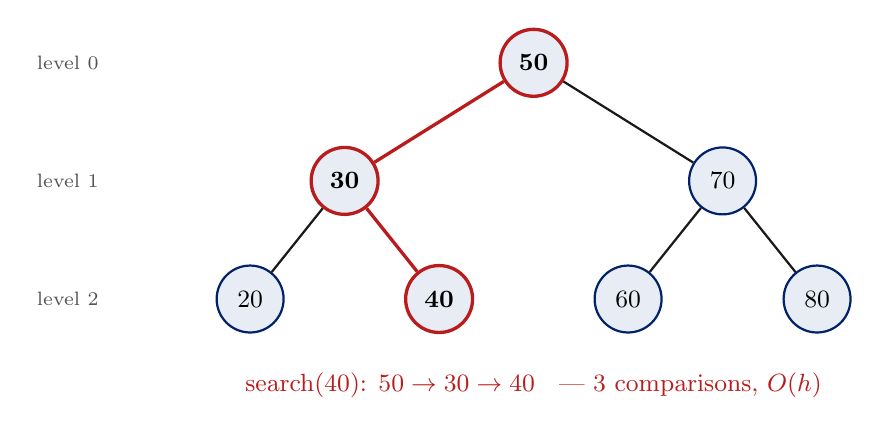
\begin{tikzpicture}

  % ---- Nodes ---------------------------------------------------------------
  \node[tnode-hi] (n50) at (4.8,  0.0) {50};
  \node[tnode-hi] (n30) at (2.4, -1.5) {30};
  \node[tnode]    (n70) at (7.2, -1.5) {70};
  \node[tnode]    (n20) at (1.2, -3.0) {20};
  \node[tnode-hi] (n40) at (3.6, -3.0) {40};
  \node[tnode]    (n60) at (6.0, -3.0) {60};
  \node[tnode]    (n80) at (8.4, -3.0) {80};

  % ---- Edges (highlighted search path drawn in red) ------------------------
  \draw[tedge-hi] (n50) -- (n30);
  \draw[tedge]    (n50) -- (n70);
  \draw[tedge]    (n30) -- (n20);
  \draw[tedge-hi] (n30) -- (n40);
  \draw[tedge]    (n70) -- (n60);
  \draw[tedge]    (n70) -- (n80);

  % ---- Level annotations ---------------------------------------------------
  \node[level-label, left] at (-0.6,  0.0) {level 0};
  \node[level-label, left] at (-0.6, -1.5) {level 1};
  \node[level-label, left] at (-0.6, -3.0) {level 2};

  % ---- Caption for the highlighted path ------------------------------------
  \node[font=\small, text=path-hi, align=center] at (4.8, -4.1)
        {search(40): $50 \to 30 \to 40$ \; --- 3 comparisons, $O(h)$};

\end{tikzpicture}
\end{document}
